\documentclass[10pt]{article}
\usepackage[polish]{babel}
\usepackage[utf8]{inputenc}
\usepackage[T1]{fontenc}
\usepackage{amsmath}
\usepackage{amsfonts}
\usepackage{amssymb}
\usepackage[version=4]{mhchem}
\usepackage{stmaryrd}
\usepackage{graphicx}
\usepackage[export]{adjustbox}
\graphicspath{ {./images/} }
\usepackage{bbold}

\title{PRACA KONTROLNA nr 1 - POZIOM PODSTAWOWY }

\author{}
\date{}


\begin{document}
\maketitle
\begin{enumerate}
  \item Ile jest liczb pięciocyfrowych podzielnych przez 9 , które w rozwinięciu dziesiętnym mają: a) obie cyfry 1, 2 i tylko te? b) obie cyfry 1,3 i tylko te? c) wszystkie cyfry 1, 2, 3 i tylko te? Odpowiedź uzasadnić. W przypadku b) wypisać otrzymane liczby.
  \item Uprościć wyrażenie $w(x)=9 x^{2}-\sqrt{\left(-9 x^{2}\right)^{2}}+3 x-\sqrt{9 x^{2}}$, a następnie:\\
a) obliczyć $w\left(\frac{\sqrt{2}-1}{\sqrt{2}+1}\right)$ oraz $w\left(\frac{1}{1-\sqrt{3}}\right)$ i wynik podać bez niewymierności w mianowniku.\\
b) wyznaczyć liczbę $b$ tak, by pole obszaru ograniczonego osiami układu współrzędnych i wykresem funkcji $f(x)=w(x)+b$ było równe 3. Sporządzić wykres funkcji $f(x)$.
  \item Sprawdzić, że liczby: $k=\frac{(\sqrt{2})^{-4}\left(\frac{1}{4}\right)^{-\frac{5}{2}} \sqrt[4]{3}}{(\sqrt[4]{16})^{3} \cdot 27^{-\frac{1}{4}}}, n=(\sqrt{3}-\sqrt{2})^{2}+(\sqrt{6}+1)^{2}$ sac całkowite i dodatnie. Wyznaczyć $m$ tak, by liczby $k, m, n$ były odpowiednio: pierwszym, drugim i trzecim wyrazem rosnącego ciągu geometrycznego. Ile trzeba wziąć początkowych wyrazów tego ciągu, by ich suma przekroczyła 100?
  \item Miejscowości $A(1,1)$ i $B(3,3)$ chcą wspólnie wybudować oczyszczalnię ścieków. Zaznaczyć na płaszczyźnie zbiór możliwych punktów umiejscowienia oczyszczalni wiedząc, że powinna ona być jednakowo oddalona od każdej z miejscowości i odległość ta nie może przekraczać 2. Ponadto odległość oczyszczalni od prostoliniowego odcinka rzeki łączącej punkty $D\left(-2,-\frac{3}{2}\right)$ i $E(4,3)$ nie powinna być mniejsza niż 1 . Rozwiązanie zilustrować rysunkiem.
  \item Jaką bryłę otrzymujemy łącząc środki ścian sześcianu? Obliczyć stosunek objętości tej bryły do objętości wyjściowego sześcianu.
  \item Wysokość opuszczona na ramię trójkąta równoramiennego dzieli jego pole w stosunku $1: 3$. Wyznaczyć tangens kąta przy podstawie oraz stosunek długości promienia okręgu wpisanego do długości promienia okręgu opisanego na tym trójkącie. Sporządzić odpowiednie rysunki.
\end{enumerate}

\section*{PRACA KONTROLNA nr 1 - POZIOM ROZSZERZONY}
\begin{enumerate}
  \item Z przystani A wyrusza z biegiem rzeki statek do przystani B, odległej od A o 140 km . Po upływie 1 godziny wyrusza za nim łódź motorowa, dopędza statek w połowie drogi, po czym wraca do przystani A w tym samym momencie, w którym statek przybija do przystani B. Wyznaczyć prędkość statku i prędkość łodzi w wodzie stojącej wiedząc, że prędkość biegu rzeki wynosi $4 \mathrm{~km} /$ godz.
  \item Niech $a(x)=\frac{\sqrt{x-1}+1}{x-2}$. Dla jakich liczb rzeczywistych $x$ zarówno wartość $a(x)$ jak i jej odwrotność są mniejsze niż 2?
  \item Wyznaczyć cosinus kąta między ścianami ośmiościanu foremnego. Obliczyć stosunek długości promienia kuli wpisanej do długości promienia kuli opisanej na tej bryle. Sporządzić odpowiednie rysunki.
  \item Liczby: $\quad a=4 \cos ^{2} \frac{\pi}{12}-\operatorname{tg} \frac{\pi}{3}, \quad b=\frac{(\sqrt[3]{2})^{54} \cdot\left(\frac{1}{\sqrt{3}}\right)^{-6}-(2 \sqrt{2})^{12} \cdot(\sqrt[3]{3})^{6}}{2^{3} \cdot\left(\sqrt[3]{\frac{1}{32}}\right)^{-12}+(4 \sqrt{2})^{8}}$ sac odpowiednio pierwszym i piątym wyrazem nieskończonego, malejącego ciągu geometrycznego. Obliczyć wyraz piętnasty oraz sumę wszystkich wyrazów tego ciągu. Ile początkowych wyrazów tego ciągu należy wziąć, by ich suma przekroczyła $85 \%$ sumy wszystkich wyrazów?
  \item Każda z przekątnych trapezu ma długość 5 , jedna z podstaw ma długość 2, a pole równe jest 12. Obliczyć promień okręgu opisanego na tym trapezie. Sporządzić rysunek.
  \item Jednym z boków trójkąta $A B C$ jest odcinek $A B$, gdzie $A(1,2), B(3,1)$. Wyznaczyć równanie zbioru wszystkich punktów $C$ takich, że kąt $B C A$ ma miarę $45^{\circ}$ oraz opisać konstrukcję wszystkich trójkątów równoramiennych spełniających warunek ten warunek. Sporządzić rysunek.
\end{enumerate}

\section*{PRACA KONTROLNA nr 2 - POZIOM PODSTAWOWY}
\begin{enumerate}
  \item Niech $A=\{(x, y):|x|+2 y \leqslant 3\}, B=\left\{(x, y):|y| \geqslant x^{2}\right\}$. Zaznaczyć na płaszczyźnie zbiory $A \cap B, A \backslash B$.
  \item Trapez o kątach przy podstawie $30^{\circ}$ oraz $45^{\circ}$ jest opisany na okręgu o promieniu $R$. Obliczyć stosunek pola koła do pola trapezu.
  \item Dla jakich wartości kąta $\alpha \in[0,2 \pi]$ równanie kwadratowe
\end{enumerate}

$$
\sin \alpha \cdot x^{2}-2 x+2 \sin \alpha-1=0
$$

ma dokładnie jedno rozwiązanie?\\
4. Pole powierzchni bocznej ostrosłupa prawidłowego trójkątnego jest 6 razy większe niż pole jego podstawy. Obliczyć cosinus kąta nachylenia krawędzi bocznej ostrosłupa do płaszczyzny podstawy.\\
5. Iloczyn dwu liczb jest 20 razy większy niż odwrotność ich sumy. Suma sześcianów tych liczb stanowi $325 \%$ iloczynu tych liczb i ich sumy. Jakie to liczby?\\
6. Narysować wykres funkcji

$$
f(x)=\left\{\begin{array}{lll}
1+x-x^{2}, & \text { gdy } & |x| \leqslant 1 \\
\frac{1}{x}, & \text { gdy } & |x|>1
\end{array}\right.
$$

a) Obliczyć $f\left(-\frac{1}{1+\sqrt{2}}\right)$ oraz $f\left(\frac{1+\sqrt{2}}{2}\right)$. Wynik podać bez niewymierności w mianowniku.\\
b) Wykorzystując wykres rozwiązać nierówność $\quad f(x) \geqslant-\frac{1}{2} \quad$ i zaznaczyć zbiór jej rozwiązań na osi $0 x$.\\
c) Odczytać z wykresu przedziały, na których funkcja $f$ jest malejąca.

\section*{PRACA KONTROLNA nr 2 - POZIOM ROZSZERZONY}
\begin{enumerate}
  \item Zaznaczyć na płaszczyźnie zbiór $\left\{(x, y):|x| \leqslant \frac{3}{2}, \log _{\frac{2}{3}}|x|<y<\log _{\frac{3}{2}}|x|\right\}$.
  \item Wykazać, że różnica kwadratów dwu dowolnych liczb całkowitych niepodzielnych przez 3 jest liczbą podzielną przez 3.
  \item W trójkącie równoramiennym $A B C$ o podstawie $A B$ ramię ma długość $b$, a kąt przy wierzchołku $C$ - miare $\gamma . D$ jest takim punktem ramienia $B C$, że odcinek $A D$ dzieli pole trójkąta na połowę. Wyznaczyć promienie okręgów wpisanych w trójkąty $A B D$ i $A D C$. Dla jakiego kąta $\gamma$ promienie te są równe?
  \item Niech $f(x)=3(x+2)^{4}+x^{2}+4 x+p$, gdzie $p$ jest parametrem rzeczywistym.\\
a) Uzasadnić, że wykres funkcji $f(x)$ jest symetryczny względem prostej $x=-2$.\\
b) Dla jakiego parametru rzeczywistego $p$ najmniejszą wartością funkcji $f(x)$ jest $y=-2$ ? Odpowiedź uzasadnić, nie stosując metod rachunku różniczkowego.\\
c) Określić liczbę pierwiastków równania $f(x)=0 \mathrm{w}$ zależności od parametru $p$.
  \item Rozwiązać nierówność $|\sin x-\sqrt{3} \cos x| \geqslant 1$.
  \item Rozwiązać równanie
\end{enumerate}

$$
1-\left(\frac{2^{x}}{3^{x}-2^{x}}\right)+\left(\frac{2^{x}}{3^{x}-2^{x}}\right)^{2}-\left(\frac{2^{x}}{3^{x}-2^{x}}\right)^{3}+\ldots=\frac{3^{x-2}}{2^{x-1}}
$$

którego lewa strona jest sumą wyrazów nieskończonego ciągu geometrycznego.

\section*{PRACA KONTROLNA nr 3 -POZIOM PODSTAWOWY}
\begin{enumerate}
  \item Boki $a_{n}$ i $b_{n}$ prostokąta $P_{n}$ są wyrazami ciągów arytmetycznych, w których $a_{1}=b_{1}=100$ oraz $r_{1}=5$ i $r_{2}=-5$. Znaleźć wszystkie wartości $n$, dla których pole prostokąta $P_{n}$ jest mniejsze o co najmniej $40 \%$ od pola prostokąta $P_{1}$.
  \item Znaleźć równania dwusiecznych kątów zawartych między prostymi $x-7 y+6=0$, $x+y-2=0$. Następnie wybrać tę dwusieczną, która tworzy z osią odciętych mniejszy kąt. Sporządzić rysunek.
  \item Pudełko zawiera 21 klocków - po 7 w kolorach żółtym, czerwonym i niebieskim. Wojtuś ułożył wieżę z 8 przypadkowo wybranych klocków. Jakie jest prawdopodobieństwo tego, że w wieży znalazły się klocki wszystkich trzech kolorów?
  \item Nie rozwiązując nierówności wykazać, że relacja
\end{enumerate}

$$
\sqrt{3 x-3 x^{2}+3}>1+\sqrt[5]{x^{2}+1}
$$

nie jest spełniona dla żadnej liczby rzeczywistej $x$.\\
5. W momencie spostrzeżenia samolotu nadlatującego ze stałą prędkością i na stałej wysokości obserwator widział go pod kątem $35^{\circ}$ do poziomu. Po jednej minucie kąt ten wzrósł do $65^{\circ}$.\\
a) Po jakim czasie od momentu spostrzeżenia samolotu przeleciał on nad głową obserwatora?\\
b) Przyjmując, że samolot leciał z prędkością $500 \mathrm{~km} / \mathrm{h}$, obliczyć na jakiej wysokości odbywał się lot.

Wyniki podać w zaokrągleniu do pełnych sekund i pełnych setek metrów.\\
6. W stożek o objętości $V$ i wysokości stanowiącej $75 \%$ promienia podstawy wpisano walec tak, że podstawa walca leży na podstawie stożka, a wysokość walca jest równa średnicy jego podstawy. Obliczyć stosunek pola powierzchni całkowitej walca do pola powierzchni całkowitej stożka oraz objętość kuli opisanej na walcu. Sporządzić odpowiedni rysunek.

\section*{PRACA KONTROLNA nr 3 -POZIOM ROZSZERZONY}
\begin{enumerate}
  \item Na diagramie składającym się z 9 kwadratowych pól w układzie $3 \times 3$ zaznaczono w losowo wybranych polach kółko i krzyżyk. Jakie jest prawdopodobieństwo tego, że oba znaki znalazły się na sąsiednich polach tzn. stykających się jednym bokiem.
  \item Kąty czworokąta wpisanego w okrąg o promieniu $R$ tworzą ciąg arytmetyczny, którego pierwszy wyraz wynosi $\frac{\pi}{4}$. Przekątna czworokąta leżąca naprzeciw kąta $\frac{\pi}{4}$ jest prostopadła do jednego z boków. Wyznaczyć kąty, obwód oraz pole tego czworokąta.
  \item Trójkąt równoramienny o podstawie $a$ i kącie przy wierzchołku $36^{\circ}$ obraca się wokół dwusiecznej kąta przy podstawie. Obliczyć objętość powstałej bryły. Skorzystać z twierdzenia o dwusiecznej kąta w trójkącie. Wynik podać bez użycia funkcji trygonometrycznych.
  \item Odcinek o końcach $A(1,1)$ i $B(3,2)$ jest bokiem prostokąta, którego jeden z wierzchołków leży na prostej $l: x-y+1=0$. Znaleźć współrzędne wierzchołków $C$ i $D$. Obliczyć cosinus kąta między przekątnymi tego prostokąta. Sporządzić rysunek.
  \item Liczba 2 jest pierwiastkiem podwójnym wielomianu $w(x)=x^{3}+a x^{2}+b x+c$, a funkcja $f(x)=w(x+1)+p$ jest nieparzysta. Znaleźć ten wielomian i obliczyć $p$. Na jednym rysunku sporządzić wykresy funkcji $f(x)$ oraz $h(x)=|w(x)|$.
  \item Wyznaczyć dziedzinę funkcji
\end{enumerate}

$$
y=\frac{\operatorname{ctg} 4 x}{\cos 2 x+\cos 6 x} .
$$

\section*{PRACA KONTROLNA nr 4 - POZIom PODSTAWOWy}
\begin{enumerate}
  \item Dane są funkcje określone wzorami $f(x)=x-3$ oraz $g(x)=4-x, x \in R$. Rozwiązać nierówność
\end{enumerate}

$$
|f(2 x-5)+g(x+1)| \leqslant\left|f\left(\frac{x}{2}-1\right)+g\left(\frac{x}{2}-4\right)\right|-2\left|g\left(\frac{x}{2}\right)\right|
$$

\begin{enumerate}
  \setcounter{enumi}{1}
  \item Wartość użytkowa pewnego urządzenia maleje z roku na rok w postępie arytmetycznym. W jakim czasie maszyna będzie całkowicie bezużyteczna, jeżeli po 25 latach pracy jej wartość była trzykrotnie mniejsza, niż jej wartość po 15 latach pracy? Po pewnych udoskonaleniach wydłużono czas użytkowania takiego urządzenia o pięć lat. O ile wolniej będzie teraz spadać jego wartość użytkowa rocznie? Wynik podać w procentach z dokładnością do jednego miejsca po przecinku.
  \item W okrąg wpisano cztery okręgi w sposób pokazany na rysunku. Wyznaczyć stosunek pola rombu, którego wierzchołkami są środki czterech wpisanych okręgów, do pola koła, w które wpisano te okręgi.\\
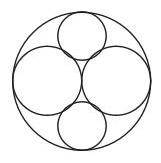
\includegraphics[max width=\textwidth, center]{2024_11_16_bc357fe772e8ec63b06ag-07}
  \item Wyznaczyć wartość parametru $a$, dla którego funkcja kwadratowa o równaniu $f(x)=(a-1) x^{2}+(a-2) x+1$ osiąga najmniejszą wartość równą 1 . Następnie znaleźć równanie prostej przechodzacej przez punkt $A(a, 2 a+1)$ prostopadłej do prostej o równaniu $4 y+x+8=0$. Jakie jest wzajemne położenie otrzymanej prostej i wykresu funkcji $f$ ? Wykonać staranny wykres funkcji $f$ oraz obu prostych.
  \item Wyznaczyć dziedzinę funkcji danej wzorem
\end{enumerate}

$$
f(x)=\frac{x-1}{\sqrt{1-\frac{2 x}{x-1}}}
$$

a następnie rozwiązać równanie $f(x)-f(-x)=2$.\\
6. W prawidłowym ostrosłupie trójkątnym ściana boczna ma pole dwa razy większe od pola podstawy. Promień kuli wpisanej w ten ostrosłup ma długość $r=1$. Obliczyć sumę wszystkich wysokości tego ostrosłupa oraz wyznaczyć tangens kąta nachylenia krawędzi bocznej do płaszczyzny podstawy.

\section*{PRACA KONTROLNA nr 4 - POZIom RozszERzony}
\begin{enumerate}
  \item Janek oszczędza na komputer i w tym celu włożył 4000 zł na lokatę roczną. Oprocentowanie tej lokaty wynosi $12 \%$ w skali roku, a odsetki kapitalizowane są co miesiąc. Jaki dochód przyniesie Jankowi ta lokata? Czy więcej uzyskałby na lokacie 18\%, w której odsetki kapitalizowane są co kwartał?
  \item Zbadać monotoniczność ciągu o wyrazach $a_{n}=\frac{1}{n+1}+\frac{1}{n+2}+\ldots+\frac{1}{n+n}$. Czy ten ciag jest ograniczony? Wyznaczyć $a_{1}, a_{2}$ i $a_{3}$.
  \item Udowodnić, stosując zasadę indukcji matematycznej, że dla każdej liczby naturalnej $n$ liczba $8^{n+1}+9^{2 n-1}$ jest podzielna przez 73 .
  \item Obliczyć sumę wszystkich tych pierwiastków równania
\end{enumerate}

$$
\sin ^{2}\left(x+\frac{\pi}{3}\right)+\cos ^{2}\left(x-\frac{\pi}{3}\right)=\frac{7}{4}
$$

które należą do przedziału $(-10,10)$.\\
5. W trójkat równoboczny $A B C$ wpisano trzy kwadraty w taki sposób, że jeden z boków każdego kwadratu zawiera się w jednym z boków trójkata. Środki tych kwadratów tworzą trójkąt równoboczny $P Q R$. Obliczyć stosunek pola trójkąta $A B C$ do pola trójkąta $P Q R$.\\
6. Krawędź kwadratowej podstawy prostopadłościanu ma długość $a$. Prostopadłościan przecięto płaszczyzną przechodzącą przez jeden z wierzchołków prostopadłościanu oraz środki dwóch sąsiednich krawędzi przeciwległej podstawy tak, że otrzymany przekrój jest pięciokątem. Obliczyć obwód oraz pole tego pięciokąta, jeżeli płaszczyzna przekroju jest nachylona do płaszczyzny podstawy pod kątem $\alpha$.

\section*{PRACA KONTROLNA nr 5 - POZIOM PODSTAWOWY}
\begin{enumerate}
  \item Biegacz wyruszył na trasę maratonu, pokonując każde 300 m w ciągu 1 minuty. Po upływie 20 minut wyruszył za nim rowerzysta i jadąc ze stałą prędkością, dogonił maratończyka dokładnie 195 m przed linią mety. Jaka była prędkość rowerzysty? Po jakim czasie powinien wyjechać rowerzysta, aby jadąc ze stałą prędkością $30 \mathrm{~km} / \mathrm{h}$, przekroczyć linię mety równocześnie z biegaczem? Wynik zaokrąglić w dół z dokładnością do 1 sekundy.
  \item Tangens kąta ostrego $\alpha$ równy jest $\frac{a}{b}$, gdzie
\end{enumerate}

$$
a=(\sqrt{2+\sqrt{3}}-\sqrt{2-\sqrt{3}})^{2}, \quad b=(\sqrt{\sqrt{2}+1}-\sqrt{\sqrt{2}-1})^{2}
$$

Wyznaczyć wartości pozostałych funkcji trygonometrycznych tego kąta. Wykorzystując wzór $\sin 2 \alpha=2 \sin \alpha \cos \alpha$, obliczyć miarę kąta $\alpha$.\\
3. W walec wpisano trzy wzajemnie styczne kule w ten sposób, że każda z nich jest styczna do ściany bocznej i obu podstaw walca. Sprawdzić, jaką część objętości walca zajmują kule. Wynik wyrażony w procentach podać z dokładnością do 1 promila.\\
4. Wskazać wszystkie te wyrazy ciągu $\left(a_{n}\right)$, gdzie

$$
a_{n}=\frac{\log _{2}^{2} n+\log _{\frac{1}{2}}\left(n^{3}\right)}{\log _{n} 2}-2 \log _{4}\left(\frac{1}{n^{2}}\right)
$$

które są równe zero.\\
5. Dwie klepsydry, mała i duża, odmierzają odpowiednio $m$ i $n, m<n$, pełnych minut. Po raz pierwszy obrócono je równocześnie w samo południe. Każdą z nich obracano, gdy tylko przesypał się w niej cały piasek. Czas mierzono do momentu, gdy obie klepsydry równocześnie przestały działać. Określić, która była wtedy godzina, jeżeli wiadomo, że małą obrócono o 13 razy więcej niż dużą, a gdy małą obracano po raz jedenasty, duża wypełniona była dokładnie w połowie.\\
6. W trójkąt równoboczny o polu $P$ wpisano okrąg oraz trzy małe okręgi - jak na rysunku. Następnie odcięto narożniki trójkąta wzdłuż łuków małych okręgów. Obliczyć pole koła opisanego na tak powstałej figurze.\\
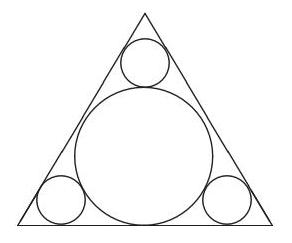
\includegraphics[max width=\textwidth, center]{2024_11_16_bc357fe772e8ec63b06ag-09}

\section*{PRACA KONTROLNA nr 5 - POZIOM ROZSZERZONY}
\begin{enumerate}
  \item Wśród prostokątów o ustalonej długości przekątnej $p$ znaleźć ten, którego pole jest największe. Nie stosować metod rachunku różniczkowego.
  \item Znaleźć wszystkie liczby rzeczywiste $m \neq 0$, dla których równanie
\end{enumerate}

$$
\frac{x}{m}+m=\frac{m}{x}+x+1
$$

ma dwa różne pierwiastki $x_{1}, x_{2}$ spełniające warunek $\left|x_{1}-x_{2}\right|>x_{1}+x_{2}$.\\
3. Rozwiązać nierówność

$$
2^{3 x-1}-2^{2 x-1}-2^{x+1}+2>0
$$

\begin{enumerate}
  \setcounter{enumi}{3}
  \item Stosując wzór na zamianę podstawy logarytmu uzasadnić, że liczba
\end{enumerate}

$$
S_{n}=\log _{m^{2^{0}}} x+\log _{m^{2^{1}}} x+\log _{m^{2^{2}}} x+\cdots+\log _{m^{2^{n}}} x, \quad \text { gdzie } x>0 \text { oraz } m \in \mathbb{N}, m>1,
$$

jest sumą częściową pewnego nieskończonego ciągu geometrycznego. Obliczyć sumę wszystkich wyrazów tego ciągu i zbadać, dla jakiego $x$ suma ta wynosi $\frac{1}{2}$.\\
5. Określić dziedzinę funkcji $f(x)=\log _{x^{2}}(1-\operatorname{tg} x \operatorname{tg} 2 x)$.\\
6. W kulę wpisano 4 identyczne małe kule wzajemnie do siebie styczne. Obliczyć, jaką część objętości dużej kuli wypełniają małe kule. Wynik wyrażony w procentach podać z dokładnością do 1 promila.

\section*{PRACA KONTROLNA nr 6 - POZIOM PODSTAWOWY}
\begin{enumerate}
  \item Obliczyć wartość wyrażenia
\end{enumerate}

$$
\frac{b^{2}-1}{a^{3}+b^{3}}:\left(\frac{a+b}{1+a b-a^{2}-a^{3} b}+\frac{1}{a+b} \cdot \frac{a b+1}{a^{2}-1}\right)
$$

dla $a=\sqrt{2}+1, b=\sqrt{2}-1$.\\
2. Pole deltoidu wpisanego w okrąg o promieniu $r$ równe jest $r^{2}$. Wyznaczyć kąty tego deltoidu.\\
3. Z miast A i B wyruszyły jednocześnie dwa samochody jadące ze stałymi prędkościami naprzeciw siebie. Do chwili spotkania pierwszy z nich przebył drogę o $d \mathrm{~km}$ większą niż drugi. Jadąc dalej z tymi samymi prędkościami, pierwszy samochód przebył drogę od A do B w $m$ godzin, drugi zaś w $n$ godzin. Obliczyć odległość między miastami A i B.\\
4. Wyznaczyć wszystkie trójkąty równoramienne o wierzchołkach $A(1,0), B(4,1)$, w których $|A B|=|A C|$ i środkowa $C D$ boku $A B$ jest zawarta w prostej $x+y=3$. Znaleźć współrzędne środka ciężkości tego z trójkątow, który ma najmniejsze pole.\\
5. Sporządzić staranny wykres funkcji $f$ zadanej wzorem

$$
f(x)=\left\{\begin{array}{lll}
\sqrt{x^{2}-4 x+4}, & \text { gdy } & \left|x-\frac{3}{2}\right| \leqslant \frac{3}{2} \\
\frac{3 x-6}{2 x-3}, & \text { gdy } & \left|x-\frac{3}{2}\right|>\frac{3}{2}
\end{array}\right.
$$

Posługując się wykresem określić zbiór wartości funkcji $f$. Wyznaczyć najmniejszą i największą wartość funkcji w przedziale $[2-\sqrt{2}, 2+\sqrt{2}]$.\\
6. W stożek wpisano graniastosłup prosty tak, że podstawa dolna graniastosłupa zawiera się w podstawie stożka, a wierzchołki górnej podstawy należą do powierzchni bocznej stożka. Podstawą graniastosłupa jest trójkąt prostokatny, w którym stosunek przyprostokątnych wynosi 1 : 3, a pole powierzchni największej ściany bocznej jest 2 razy mniejsze niż pole przekroju osiowego stożka. Obliczyć stosunek objętości graniastosłupa do objętości stożka.

\section*{PRACA KONTROLNA nr 6 - POZIOM ROZSZERZONY}
\begin{enumerate}
  \item Sporządzić staranny wykres funkcji $f(x)=\left|2^{\frac{3-|x|}{2}}-1\right|$. Opisać i uzasadnić sposób postępowania.
  \item Rozwiązać nierówność
\end{enumerate}

$$
\frac{\sqrt{x^{2}-1}}{x} \leqslant \frac{\sqrt{6 x+36}}{8}
$$

\begin{enumerate}
  \setcounter{enumi}{2}
  \item Punkty $K, L, M$ dzielą odpowiednio boki $A B, B C, C A$ trójkąta w stosunku $1: 3$ oraz $\overrightarrow{A B}=[11,2], \overrightarrow{A C}=[2,4]$. Posługując się rachunkiem wektorowym, obliczyć cosinus kąta $\angle M K L$.
  \item Wyznaczyć wszystkie wartości parametru całkowitego $m$, dla których para liczb $(x, y)$ spełniająca układ równań
\end{enumerate}

$$
\left\{\begin{array}{l}
2 x+y=4 \\
4 x+3 y=m
\end{array}\right.
$$

jest rozwiązaniem nierówności $x-\sqrt{8} y \leqslant 4$ oraz $x \log _{3} 2+y \log _{3} 5 \leqslant x \log _{3} 7$.\\
5. Podstawą ostrosłupa czworokątnego jest prostokąt o przekątnej długości $d$, a wszystkie krawędzie boczne mają tę samą długość. Większa ściana boczna jest nachylona do podstawy pod kątem $\alpha$, a mniejsza pod kątem $\beta$. Obliczyć objętość i pole powierzchni bocznej ostrosłupa.\\
6. Dany jest układ równań

$$
\left\{\begin{array}{l}
x-3|y+1|=0 \\
(x-p)^{2}+y^{2}=5
\end{array}\right.
$$

gdzie $p$ jest parametrem rzeczywistym.\\
a) Rozwiązać algebraicznie powyższy układ dla $p=2$ i podać jego interpretację geometryczną. Sporządzić rysunek.\\
b) Korzystając z rysunku i odpowiednich rozważań geometrycznych, określić liczbę rozwiązań danego układu w zależności od parametru $p$.


\end{document}